\section{Phân tích yêu cầu}

%Section 2.1 (old): Problem description
%Nội dung chương này hoàn toàn được bao hàm bên trong lý do chọn đề tài cũng như mục tiêu đề tài. Nên QC lược bớt.

%Section 2.1 (new): Stakeholders and their benefit
%Dời chương 2.3 lên này
\subsection{Phân tích các bên liên quan}

Việc phát triển và triển khai Hệ thống Thương mại Điện tử cho Bán lẻ Điện thoại tích hợp Trợ lý Ảo AI Agent là một bước tiến công nghệ quan trọng, mang lại những lợi ích thiết thực và giá trị gia tăng rõ rệt cho các bên liên quan trực tiếp đến hoạt động kinh doanh và vận hành hệ thống. 

\subsubsection{Khách hàng}

Ở cấp độ quản lý, hệ thống này đóng vai trò then chốt trong việc củng cố khả năng cạnh tranh của doanh nghiệp trên thị trường số. Việc cung cấp trải nghiệm AI tiên tiến giúp thu hút và giữ chân khách hàng, đồng thời tăng tỷ lệ chuyển đổi đơn hàng thông qua gợi ý cá nhân hóa. Về mặt kỹ thuật, hệ thống đảm bảo tính ổn định, bảo mật và khả năng mở rộng, giúp doanh nghiệp giảm thiểu rủi ro vận hành và dễ dàng phát triển dịch vụ trong tương lai mà không cần thay đổi kiến trúc cốt lõi.

\subsubsection{Đội ngũ vận hàng và quản trị viên}

Đối với đội ngũ nội bộ, hệ thống mới giúp tăng hiệu suất làm việc và tối ưu hóa quy trình quản lý. Lợi ích chính là việc tự động hóa khâu chăm sóc khách hàng, giúp đội ngũ hỗ trợ giảm tải khối lượng câu hỏi thường gặp. Quản trị viên có được một giao diện tập trung để quản lý sản phẩm, giá cả và khuyến mãi hiệu quả. Hơn nữa, hệ thống cung cấp báo cáo cơ bản và cơ chế cập nhật trạng thái đơn hàng, hỗ trợ công tác quản lý và ra quyết định.

\subsubsection{Chủ sở hữu doanh nghiệp}

Ở cấp độ quản lý, hệ thống này đóng vai trò then chốt trong việc củng cố khả năng cạnh tranh của doanh nghiệp trên thị trường số. Việc cung cấp trải nghiệm AI tiên tiến giúp thu hút và giữ chân khách hàng, đồng thời tăng tỷ lệ chuyển đổi đơn hàng thông qua gợi ý cá nhân hóa. Về mặt kỹ thuật, hệ thống đảm bảo tính ổn định, bảo mật và khả năng mở rộng, giúp doanh nghiệp giảm thiểu rủi ro vận hành và dễ dàng phát triển dịch vụ trong tương lai mà không cần thay đổi kiến trúc cốt lõi.

\subsubsection{Nhóm phát triển đề tài}

Dự án là nền tảng để nhóm phát triển ứng dụng và kiểm chứng các kỹ thuật hiện đại, đặc biệt là trong lĩnh vực Xử lý Ngôn ngữ Tự nhiên (NLP) và thiết kế kiến trúc vi dịch vụ cho thương mại điện tử. Lợi ích là kinh nghiệm thực tiễn trong việc tích hợp thành công công nghệ AI vào một hệ thống giao dịch phức tạp, tạo ra một sản phẩm minh chứng có giá trị nghiên cứu và ứng dụng cao.

Từ việc phân tích các bên liên quan, có thể thấy nhu cầu của từng nhóm được cụ thể hóa rõ ràng và gắn liền với vai trò mà họ đảm nhận trong hệ thống.Những nhu cầu trên chính là cơ sở để xác định các yêu cầu chức năng của hệ thống, bao gồm tính năng tìm kiếm, giỏ hàng, thanh toán mô phỏng, trợ lý ảo kịch bản và quản trị sản phẩm. Song song, các yêu cầu phi chức năng ở mức tối thiểu như sự ổn định cho bản demo, tốc độ phản hồi hợp lý và bảo mật thông tin người dùng cũng cần được đảm bảo để hệ thống có thể vận hành hiệu quả trong phạm vi nghiên cứu.

%Section 2.2
\subsection{Khảo sát thị trường}
Trong giai đoạn đầu của quá trình phát triển đề tài, nhóm tiến hành khảo sát thực tế các nền tảng thương mại điện tử phổ biến tại Việt Nam trong lĩnh vực bán lẻ điện thoại và thiết bị công nghệ như: CellphoneS, FPT Shop và Thế Giới Di Động. Mục tiêu của quá trình khảo sát là đánh giá chức năng cốt lõi, trải nghiệm người dùng (UI/UX), và đặc biệt là khả năng hỗ trợ khách hàng thông qua chatbot hoặc trợ lý ảo của các hệ thống hiện có.

Kết quả khảo sát cho thấy các nền tảng này đều đã xây dựng hệ thống thương mại điện tử hiện đại, có giao diện trực quan, quy trình mua hàng rõ ràng và khả năng tra cứu sản phẩm nhanh chóng. Người dùng có thể dễ dàng xem thông tin chi tiết, so sánh giá, đặt hàng và thanh toán trực tuyến. Tuy nhiên, khi đi sâu vào khả năng hỗ trợ thông minh, nhóm nhận thấy rằng đa số các hệ thống hiện nay vẫn hoạt động dựa trên cơ chế tương tác truyền thống, chủ yếu yêu cầu người dùng thao tác thủ công để thực hiện tìm kiếm hoặc truy vấn thông tin.

Một số nền tảng như CellphoneS và Thế Giới Di Động đã tích hợp chatbot hỗ trợ khách hàng, tuy nhiên các chatbot này chỉ dừng lại ở mức trả lời câu hỏi hoặc hướng dẫn cơ bản, chẳng hạn như cung cấp thông tin khuyến mãi, tra cứu đơn hàng qua mã đơn, hoặc tư vấn sản phẩm theo từ khóa có sẵn. Các chatbot chưa thể hiểu được ngữ cảnh người dùng, không có khả năng ghi nhớ trạng thái hội thoại, và chưa thực hiện được các hành động trực tiếp trên hệ thống như đặt hàng, thêm sản phẩm vào giỏ, hoặc hủy đơn.

\begin{figure}[H]
\centering
\begin{minipage}{0.48\textwidth}
    \centering
    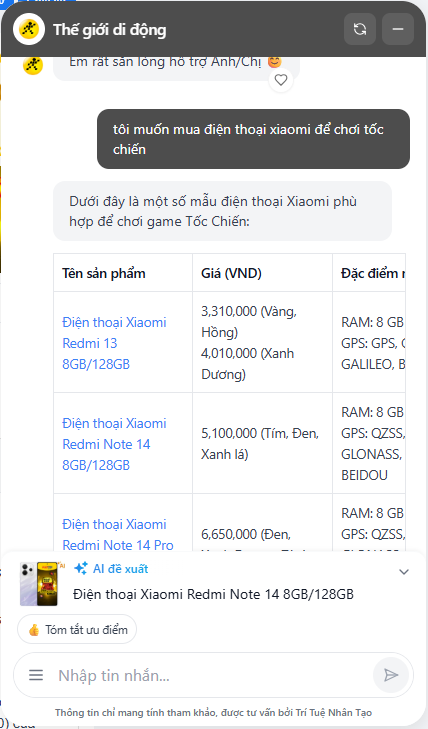
\includegraphics[width=0.8\textwidth]{images/khao_sat_thi_truong/tgdd-good.png}
\end{minipage}
\hfill
\begin{minipage}{0.48\textwidth}
    \centering
    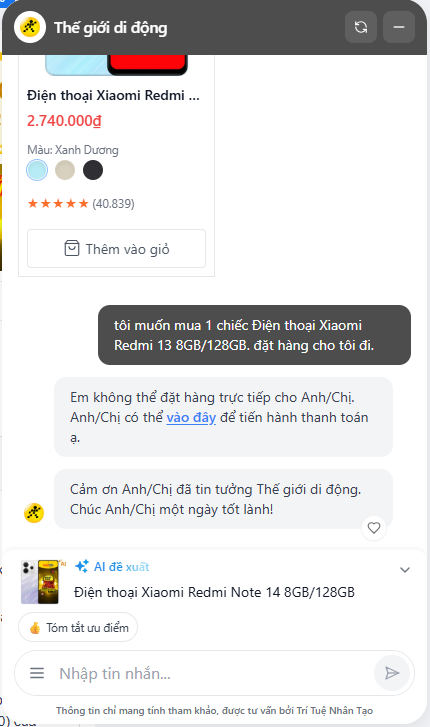
\includegraphics[width=0.8\textwidth]{images/khao_sat_thi_truong/tgdd-bad.png}
\end{minipage}
\vspace{0.5cm}
\caption{Trợ lý ảo của Thế Giới Di Động}
\end{figure}

Đối với FPT Shop, hệ thống hỗ trợ khách hàng chủ yếu được triển khai dưới dạng cửa sổ trò chuyện với nhân viên tư vấn trực tuyến cho các tác vụ tương tác sâu như kiểm tra thông tin giỏ hàng và các đơn hàng đã đặt, thay vì chatbot tự động. Cách tiếp cận này giúp tăng tính chính xác trong phản hồi, song không đảm bảo khả năng phản hồi nhanh và tự động hóa quy trình chăm sóc khách hàng khi lưu lượng truy cập tăng cao.

\begin{figure}[H]
\centering
\begin{minipage}{0.48\textwidth}
    \centering
    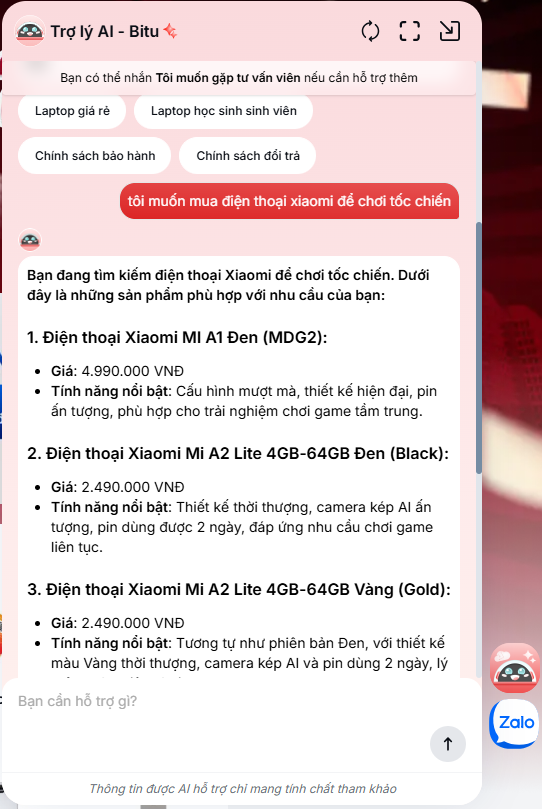
\includegraphics[width=0.8\textwidth]{images/khao_sat_thi_truong/fpt-good.png}
\end{minipage}
\hfill
\begin{minipage}{0.48\textwidth}
    \centering
    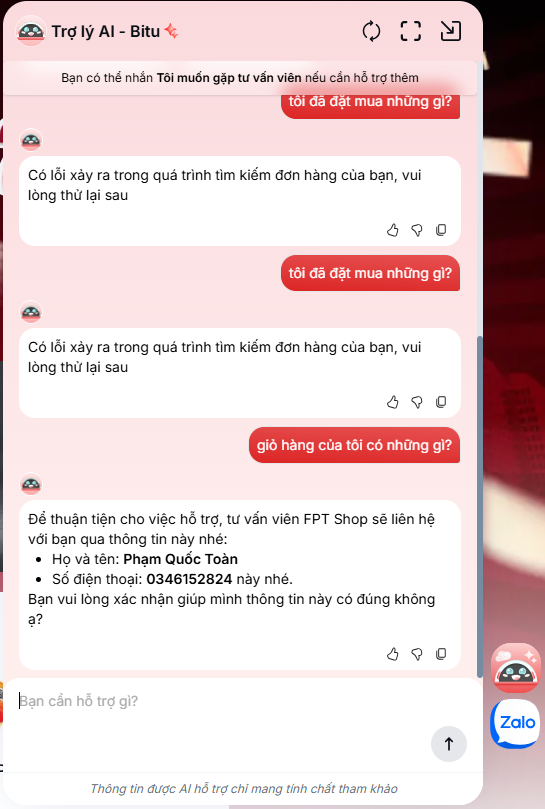
\includegraphics[width=0.8\textwidth]{images/khao_sat_thi_truong/fpt-bad.png}
\end{minipage}
\vspace{0.5cm}
\caption{Trợ lý ảo của FPT Shop}
\end{figure}

Qua kết quả khảo sát, nhóm nhận thấy rằng mặc dù các doanh nghiệp trong ngành đã có bước tiến lớn trong việc số hóa hoạt động bán lẻ, chưa có nền tảng nào tại Việt Nam tích hợp Trợ lý Ảo thông minh có khả năng giao tiếp tự nhiên và thực hiện hành động thực tế trên hệ thống. Khoảng trống này mở ra cơ hội để nhóm nghiên cứu và phát triển một mô hình thương mại điện tử tích hợp Trợ lý Ảo AI Agent, hướng đến việc nâng cao trải nghiệm người dùng, tự động hóa quy trình giao dịch, và tăng tính cá nhân hóa trong tương tác mua sắm.

%Section 2.3: Fuctional requirement
\subsection{Yêu cầu chức năng}

 \subsubsection{Đối với khách hàng}

\begin{itemize}

\item \textbf{[FR1] Đăng ký} \hfill (\textit{Ưu tiên: Cao})\\
    Cho phép khách hàng tự đăng ký tài khoản mới và quản lý thông tin cá nhân. Tài khoản quản trị viên được hệ thống cấp riêng và không thể tự đăng ký.

\item \textbf{[FR2] Đăng nhập/Đăng xuất} \hfill (\textit{Ưu tiên: Trung Bình})\\
    Cho phép khách hàng đăng nhập bằng tài khoản đã đăng ký (email/số điện thoại và mật khẩu) và đăng xuất khỏi hệ thống.

\item \textbf{[FR3] Đăng nhập Google} \hfill (\textit{Ưu tiên: Cao})\\
    Hỗ trợ đăng nhập bằng tài khoản Google.

\item \textbf{[FR4] Quên mật khẩu} \hfill (\textit{Ưu tiên: Trung bình})\\
    Cung cấp cho khách hàng phương thức lấy lại mật khẩu trong trường hợp khách hàng quên mật khẩu.

\item \textbf{[FR5] Quản lí hồ sơ} \hfill (\textit{Ưu tiên: Thấp})\\
    Cho phép khách hàng thêm và sửa đổi hồ sơ thông tin cá nhân của bản thân.

\item \textbf{[FR6] Tìm kiếm và lọc} \hfill (\textit{Ưu tiên: Cao})\\
    Cung cấp chức năng tìm kiếm sản phẩm theo tên và lọc sản phẩm theo tiêu chí như giá, cấu hình và khuyến mãi.

\item \textbf{[FR7] Giỏ hàng và thanh toán} \hfill (\textit{Ưu tiên: Cao})\\
    Cho phép khách hàng thêm sản phẩm vào giỏ hàng, chỉnh sửa và tiến hành thanh toán.

\item \textbf{[FR8] Đa phương thức thanh toán} \hfill (\textit{Ưu tiên: Trung bình})\\
    Hỗ trợ đa phương thức thanh toán, bao gồm thẻ ngân hàng và ví điện tử.

\item \textbf{[FR9] Thông tin sản phẩm minh bạch} \hfill (\textit{Ưu tiên: Cao})\\
    Hiển thị thông tin chi tiết sản phẩm, giá cả, tình trạng tồn kho và phương thức thanh toán minh bạch.
    Hỗ trợ hiển thị sản phẩm theo phân trang để đảm bảo tốc độ tải và trải nghiệm người dùng.

\item \textbf{[FR10] Hủy đơn hàng} \hfill (\textit{Ưu tiên: Trung bình})\\
    Cho phép khách hàng hủy đơn hàng nếu đơn hàng đáp ứng được các điều kiện ràng buộc.

\item \textbf{[FR11] Trợ lý Ảo (Tìm kiếm/gợi ý)} \hfill (\textit{Ưu tiên: Cao})\\
    Trợ lý ảo hỗ trợ khách hàng tìm kiếm sản phẩm theo ngôn ngữ tự nhiên và gợi ý sản phẩm phù hợp dựa trên nhu cầu, sở thích và ngân sách.

\item \textbf{[FR12] Trợ lý Ảo (Tư vấn FAQ)} \hfill (\textit{Ưu tiên: Cao})\\
    Trợ lý ảo cung cấp tư vấn cơ bản và trả lời câu hỏi thường gặp, bao gồm chính sách bảo hành, đổi trả, khuyến mãi và phương thức thanh toán.

\item \textbf{[FR13] Trợ lý Ảo (Hỗ trợ sau mua)} \hfill (\textit{Ưu tiên: Trung bình})\\
    Trợ lý ảo đồng hành sau mua hàng, hỗ trợ khách hàng tra cứu trạng thái đơn hàng, nhắc nhở xác nhận giao dịch và thu thập phản hồi trải nghiệm.

\item \textbf{[FR14] Lịch sử \& Theo dõi đơn hàng} \hfill (\textit{Ưu tiên: Cao})\\
    Cho phép khách hàng xem lịch sử đơn hàng và theo dõi trạng thái đơn hàng đang xử lý hoặc vận chuyển.

\item \textbf{[FR15] Đánh giá} \hfill (\textit{Ưu tiên: Trung bình})\\
    Cho phép khách hàng gửi đánh giá cho sản phẩm sau khi hoàn thành đơn hàng.

\end{itemize}

\subsubsection{Đối với quản trị viên}

\begin{itemize}
    \item \textbf{[FR16] Phân quyền Người dùng} \hfill (\textit{Ưu tiên: Cao})\\
    Phân quyền giữa khách hàng và quản trị viên, đảm bảo mỗi nhóm có quyền truy cập và thao tác phù hợp với vai trò của mình trong hệ thống.

\item \textbf{[FR17] Quản lý Sản phẩm} \hfill (\textit{Ưu tiên: Cao})\\
    Giao diện quản trị cho phép thêm, chỉnh sửa, xóa sản phẩm, cập nhật giá và quản lý các chương trình khuyến mãi.

\item \textbf{[FR18] Báo cáo Cơ bản} \hfill (\textit{Ưu tiên: Trung bình})\\
    Hệ thống cung cấp báo cáo cơ bản cho quản trị viên, bao gồm tổng quan về số lượng đơn hàng, doanh thu mô phỏng và danh sách các sản phẩm bán chạy nhất.

\item \textbf{[FR19] Cập nhật Trạng thái Đơn hàng} \hfill (\textit{Ưu tiên: Cao})\\
    Tự động cập nhật thông tin trạng thái đơn hàng dựa trên dữ liệu tích hợp từ đơn vị vận chuyển (hoặc dữ liệu nhập tay của admin), đảm bảo thông tin chính xác đến khách hàng.
    
\end{itemize}
%Section 2.4: Non-Fuctional requirement
 \subsection{Yêu cầu phi chức năng}

\subsubsection{Đối với khách hàng}

\begin{itemize}

\item \textbf{[NFR1] Hiệu năng của phản hồi chung} \hfill (\textit{Ưu tiên: Cao})\\
    Thời gian phản hồi của hệ thống (cho các tác vụ không liên quan đến trợ lý ảo) không vượt quá 3 giây trong điều kiện tải bình thường.

\item \textbf{[NFR2] Hiệu năng trợ lý ảo} \hfill (\textit{Ưu tiên: Cao})\\
    Thời gian phản hồi của trợ lý ảo khi trả lời câu hỏi hoặc gợi ý sản phẩm không vượt quá 5 giây.

\item \textbf{[NFR3] Đơn giản hóa giao diện} \hfill (\textit{Ưu tiên: Cao})\\
    Giao diện người dùng phải thân thiện, cho phép khách hàng hoàn thành thao tác đặt hàng cơ bản trong tối đa 5 bước.

\item \textbf{[NFR4] Khả năng dẫn dắt khách hàng} \hfill (\textit{Ưu tiên: Trung bình})\\
    Trợ lý ảo có khả năng hướng dẫn khách hàng mới sử dụng hệ thống thành thạo trong tối đa 3 lần tương tác.

\item \textbf{[NFR5] Dễ dàng học cách dùng} \hfill (\textit{Ưu tiên: Cao})\\
    Người dùng có thể học cách sử dụng các chức năng chính như tìm kiếm, so sánh, giỏ hàng, thanh toán chỉ sau 2 lần thử nghiệm thực tế.

\item \textbf{[NFR6] Chất lượng giao tiếp của trợ lý ảo} \hfill (\textit{Ưu tiên: Cao})\\
    Trợ lý ảo cần sử dụng ngôn ngữ tự nhiên dễ hiểu, tránh thuật ngữ kỹ thuật, đảm bảo 80\% câu trả lời ở mức chấp nhận được theo đánh giá từ nhóm thử nghiệm nội bộ.

\end{itemize}

\subsubsection{Đối với quản trị viên và nhóm kỹ thuật}

\begin{itemize}
    \item \textbf{[NFR7] Độ ổn định dịch vụ} \hfill (\textit{Ưu tiên: Trung bình})\\
    Hệ thống cần duy trì hoạt động ổn định; tỷ lệ gián đoạn dịch vụ (downtime) không được vượt quá 1\% tổng thời gian hoạt động trong suốt giai đoạn thử nghiệm/demo.

\item \textbf{[NFR8] Bảo mật dữ liệu người dùng} \hfill (\textit{Ưu tiên: Cao})\\
    Hệ thống phải bảo vệ thông tin cá nhân của người dùng bằng cách mã hóa dữ liệu nhạy cảm và tuyệt đối không lưu trữ mật khẩu dưới dạng văn bản rõ ràng.

\item \textbf{[NFR9] Khả năng mở rộng} \hfill (\textit{Ưu tiên: Trung bình})\\
    Thiết kế hệ thống phải linh hoạt, cho phép tích hợp thêm các tính năng mới như phương thức thanh toán hoặc dịch vụ giao hàng mà không cần thay đổi kiến trúc tổng thể của ứng dụng.

\item \textbf{[NFR10] Hiệu suất báo cáo admin} \hfill (\textit{Ưu tiên: Thấp})\\
    Giao diện quản trị phải hiển thị các báo cáo tổng hợp (ví dụ: 1000 đơn hàng) trong vòng 5 giây để đảm bảo hiệu quả cho việc thử nghiệm và đánh giá hệ thống.

\item \textbf{[NFR11] Tính toàn vẹn} \hfill (\textit{Ưu tiên: Cao})\\
    Hệ thống phải đảm bảo cơ chế đồng bộ hóa dữ liệu khi xử lý đặt hàng để ngăn chặn tình trạng số lượng sản phẩm bị âm. Cần có biện pháp kiểm soát tính nhất quán giữa dữ liệu cache và cơ sở dữ liệu gốc (nếu có).

\end{itemize}



%Section 2.5: Use case diagram and format table
\input{contents/chap2/5_use_case}

%Section 2.6, 2.7: @TranNguyeAnhKhoa viết tiếp nhó
\input{contents/chap2/6_activity_diagram}
\input{contents/chap2/7_sequence_diagram}
